\section{QPRESENT}

\begin{frame}{QPRESENT\footfullcite{gop}}
\begin{itemize}
    \item Authors used LIGHTER-R tool \cite{LighterR}\footfullcite{LighterR} for optimized implementation of Sbox with no ancilla qubits 
    \begin{figure}[h!]
    \centering
    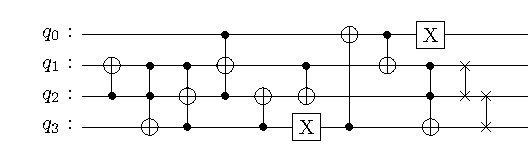
\includegraphics[width=\linewidth]{present/sbox.pdf}
    \caption{Sbox for QPRESENT}
    \label{fig:qpsbox}
\end{figure}
\pause
\item Permutation layer can be implemented using only SWAP gates. The quantum cost for the permutation layer of QPRESENT is zero.
\end{itemize}
\end{frame}
\begin{frame}{Key schedule Algorithm}
    The input is an 80-bit key and the output is a 64-bit round key.
    \pause
    \begin{codebox}
\Procname{$\proc{Key Expansion for QPRESENT}(K = k_{79}k_{78}$..$k_0)$}\label{proc:keqp}
\li $k = \mathrm{k_{63}}\mathrm{k_{62}}..\mathrm{k_{0s}} = k_{79}k_{78}..k_{16}$
\li $k \gets k \gg 19$
\li $[k_{79}k_{78}k_{77}k_{76}] = S[k_{79}k_{78}k_{77}k_{76}]$
\li $[k_{19}k_{18}k_{17}k_{16}k_{15}] = X[k_{19}k_{18}k_{17}k_{16}k_{15}]$
\li \Return $k$
\end{codebox}
 Instead of rotating 61 bits to left, rotate 19 bits to right using SWAP gates.
\end{frame}
\begin{frame}{Grover's Attack and Cost Estimates}
    Similar to Grover's Attack on SIMON
    \begin{figure}[h!]
    \centering
    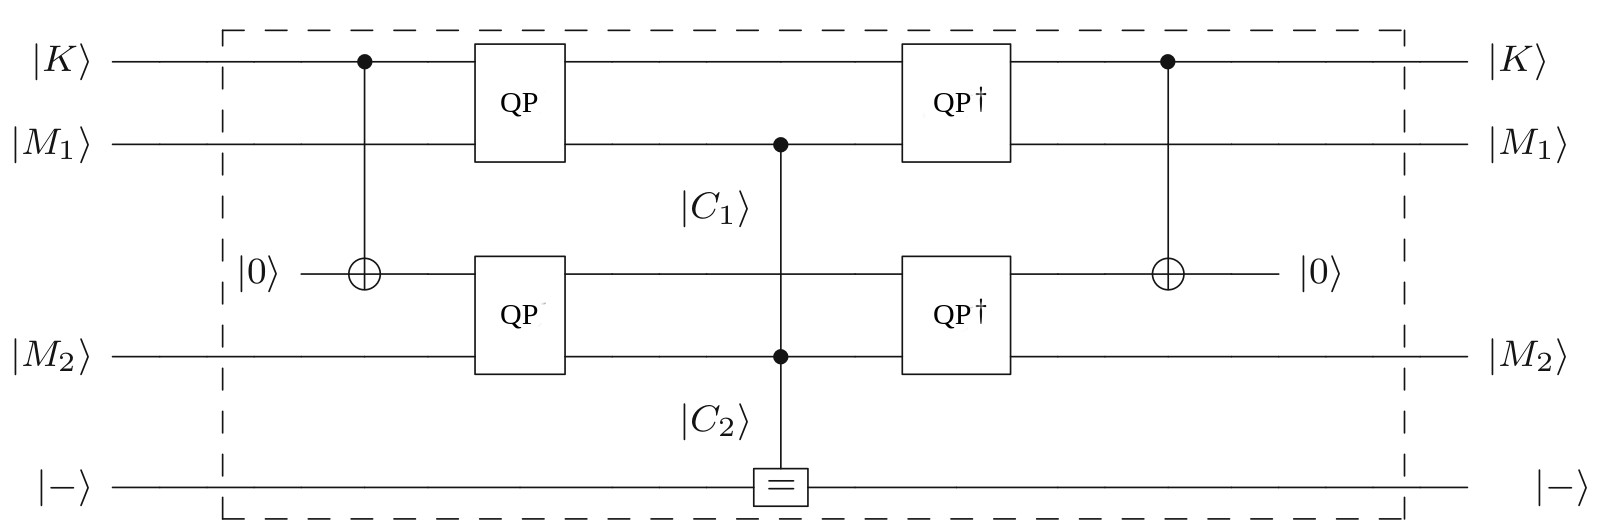
\includegraphics[width=\linewidth]{present/qpgrov.jpg}
    \caption{Grover's Attack on QPRESENT for r = 2}
    \label{fig:qpgrov}
\end{figure}
\begin{center}
\pause
\begin{table}[h!]
    \centering
    \begin{tabular}{ |c|c|c|c|c|c|c|c| } 
     \hline
     Cipher  & Qubits & X & CX & CCX & Ancilla & Depth \\ \hline
     QPRESENT 64/80 & 144 & 1118 & 4683 & 2108 & - & 311 \\ \hline
     QSIMON 64/128 & 192 &1216 & 7396 & 1408 & - & 2643\\ \hline
    \end{tabular}
    \caption{Comparison of cost for QPRESENT 64/80 \cite{gop} and QSIMON 64/128\cite{gos} }
    \label{tab:cqpqs}
\end{table}
\end{center}
\end{frame}